\documentclass[11pt]{article}
\usepackage[margin=0.92in]{geometry}
\usepackage[T1]{fontenc}
\usepackage[utf8]{inputenc}
\usepackage{array}
\usepackage{graphicx}
\usepackage{booktabs}
\usepackage{amsmath}
\usepackage{caption}
\usepackage{float}
\usepackage{hyperref}
\usepackage{xurl}
\usepackage{xcolor}
\graphicspath{{figures/}}
\hypersetup{colorlinks=true, linkcolor=blue!45!black, urlcolor=blue!45!black, citecolor=blue!45!black}
\setlength{\parindent}{0pt}
\setlength{\parskip}{0.55em}
\setlength{\emergencystretch}{3em}
\captionsetup{font=small, labelfont=bf}
% Auto-generated by generate_no_training_report.py; do not edit by hand.
\newcommand{\MatchedKalshiRecords}{3,899}
\newcommand{\CandidateNewsItems}{232,647}
\newcommand{\PositivePosteriorRecords}{1,513}
\newcommand{\PositivePosteriorRate}{38.8\%}
\newcommand{\JoinedDomains}{388}
\newcommand{\MBFCMatchedDomains}{274}
\newcommand{\TrancoMatchedDomains}{379}
\newcommand{\IffyFlaggedDomains}{10}
\newcommand{\PriorAlignmentPositive}{0.585}
\newcommand{\PriorWastePositive}{0.415}
\newcommand{\PriorTopPositiveRate}{70.2\%}
\newcommand{\PriorExactTopRate}{20.8\%}
\newcommand{\TestPriorAlignmentPositive}{0.505}
\newcommand{\TestPriorTopPositiveRate}{61.9\%}
\newcommand{\TestPriorExactTopRate}{16.2\%}
\newcommand{\TrancoPosteriorSpearman}{0.353}
\newcommand{\TrancoPriorSpearman}{0.360}
\newcommand{\MBFCTrafficPosteriorSpearman}{0.356}
\newcommand{\MBFCCredibilityPosteriorSpearman}{-0.208}
\newcommand{\MBFCCredibilityPriorSpearman}{-0.152}
\newcommand{\ItemPositiveRecordSpearman}{0.086}
\newcommand{\TestItemPositiveRecordSpearman}{0.067}
\newcommand{\WithinRecordSpearmanMean}{0.153}
\newcommand{\TestWithinRecordSpearmanMean}{0.084}
\newcommand{\DomainPriorPosteriorSpearman}{0.532}
\newcommand{\DomainPriorPosteriorPearson}{0.438}
\newcommand{\RandomTopOneZeroMissRate}{72.9\%}

\title{Attention Proxies in SWM Kalshi News Attributions}
\author{Prediction-market exploratory analysis}
\date{June 16, 2026}
\begin{document}
\maketitle
\begin{abstract}
This memo asks whether external source attributes help identify news that is useful for prediction-market belief updates in the released Social World Model (SWM) Kalshi data. The main result is source-level: popularity and traffic are positive correlates of posterior helpfulness, while raw credibility labels are not. Tranco attention correlates with posterior helpfulness at Spearman \TrancoPosteriorSpearman, and MBFC traffic is similar (\MBFCTrafficPosteriorSpearman). MBFC credibility is negative in the unadjusted domain panel (\MBFCCredibilityPosteriorSpearman), a descriptive pattern that is likely confounded by source and category mix. A second diagnostic explains why source-level patterns should not be read as item-level explanations: on held-out Kalshi records, item-level prior attention and posterior helpfulness have Spearman correlation only \TestItemPositiveRecordSpearman\ among records with any posterior-positive news.
\end{abstract}
\section{Objective and Short Answer}
The broader project asks whether prediction-market rationales that attract attention are also the rationales that add predictive information. The SWM release does not contain community rationales or comment engagement. It does contain candidate news, learned prior-attributor scores, and hindsight/posterior attribution scores. This report therefore tests the closest available source-level analogue.
\begin{itemize}
\item Popularity is the clearest external correlate. Tranco attention and MBFC traffic are positively associated with posterior helpfulness and prior attention.
\item Credibility is not positively associated with helpfulness in the raw panel. MBFC credibility is negative for both posterior helpfulness and prior attention, but this is descriptive and likely confounded.
\item The SWM prior attributor helps interpret these source patterns but is not a faithful item-level explanation. In held-out positive records, exact top-item recovery is only \TestPriorExactTopRate.
\end{itemize}
\section{What the SWM Scores Mean}
The SWM paper models prediction-market prices as social beliefs and news articles as possible events that move those beliefs. For each market transition, the paper uses two attribution models. A posterior attributor $Q_\phi$ sees the realized next state and assigns hindsight responsibility to candidate news. A prior attributor $P_\eta$ sees only the current market context and candidate news, and is trained to approximate the posterior weights. In the released files used here, $s_{ri}$ is the posterior/hindsight score for news item $i$ in record $r$, and $q_{ri}$ is the prior-attributor score for that same item.
\begin{align}
q_{ri} &= P_\eta(Z_r=i \mid s_r,E_r),\\
H_d &= \frac{1}{N_d}\sum_{(r,i):d_{ri}=d}s_{ri},\qquad
A_d = \frac{1}{N_d}\sum_{(r,i):d_{ri}=d}q_{ri}.
\end{align}
$H_d$ is a domain's average hindsight helpfulness, and $A_d$ is the average learned prior attention assigned to that domain. The analysis uses \MatchedKalshiRecords\ matched Kalshi records and \CandidateNewsItems\ candidate news items. \PositivePosteriorRecords\ records (\PositivePosteriorRate) have at least one positive posterior attribution. We join article domains to Tranco popularity ranks, MBFC-derived traffic and credibility fields, and Iffy flags.
\section{Finding 1: Popularity Is Clearer Than Credibility}
External source attributes add a second distinction. Popularity measures are positive correlates of both posterior helpfulness and prior attention: Tranco attention has Spearman \TrancoPosteriorSpearman\ with posterior helpfulness and \TrancoPriorSpearman\ with prior attention. MBFC traffic is similar for posterior helpfulness (\MBFCTrafficPosteriorSpearman). By contrast, MBFC credibility is negative in the raw domain panel (\MBFCCredibilityPosteriorSpearman\ with posterior helpfulness and \MBFCCredibilityPriorSpearman\ with prior attention). This does not mean credibility causes lower usefulness. The domain panel is confounded by category mix, source mix, and what kinds of events happened to move Kalshi prices in the release.
\begin{figure}[H]
\centering
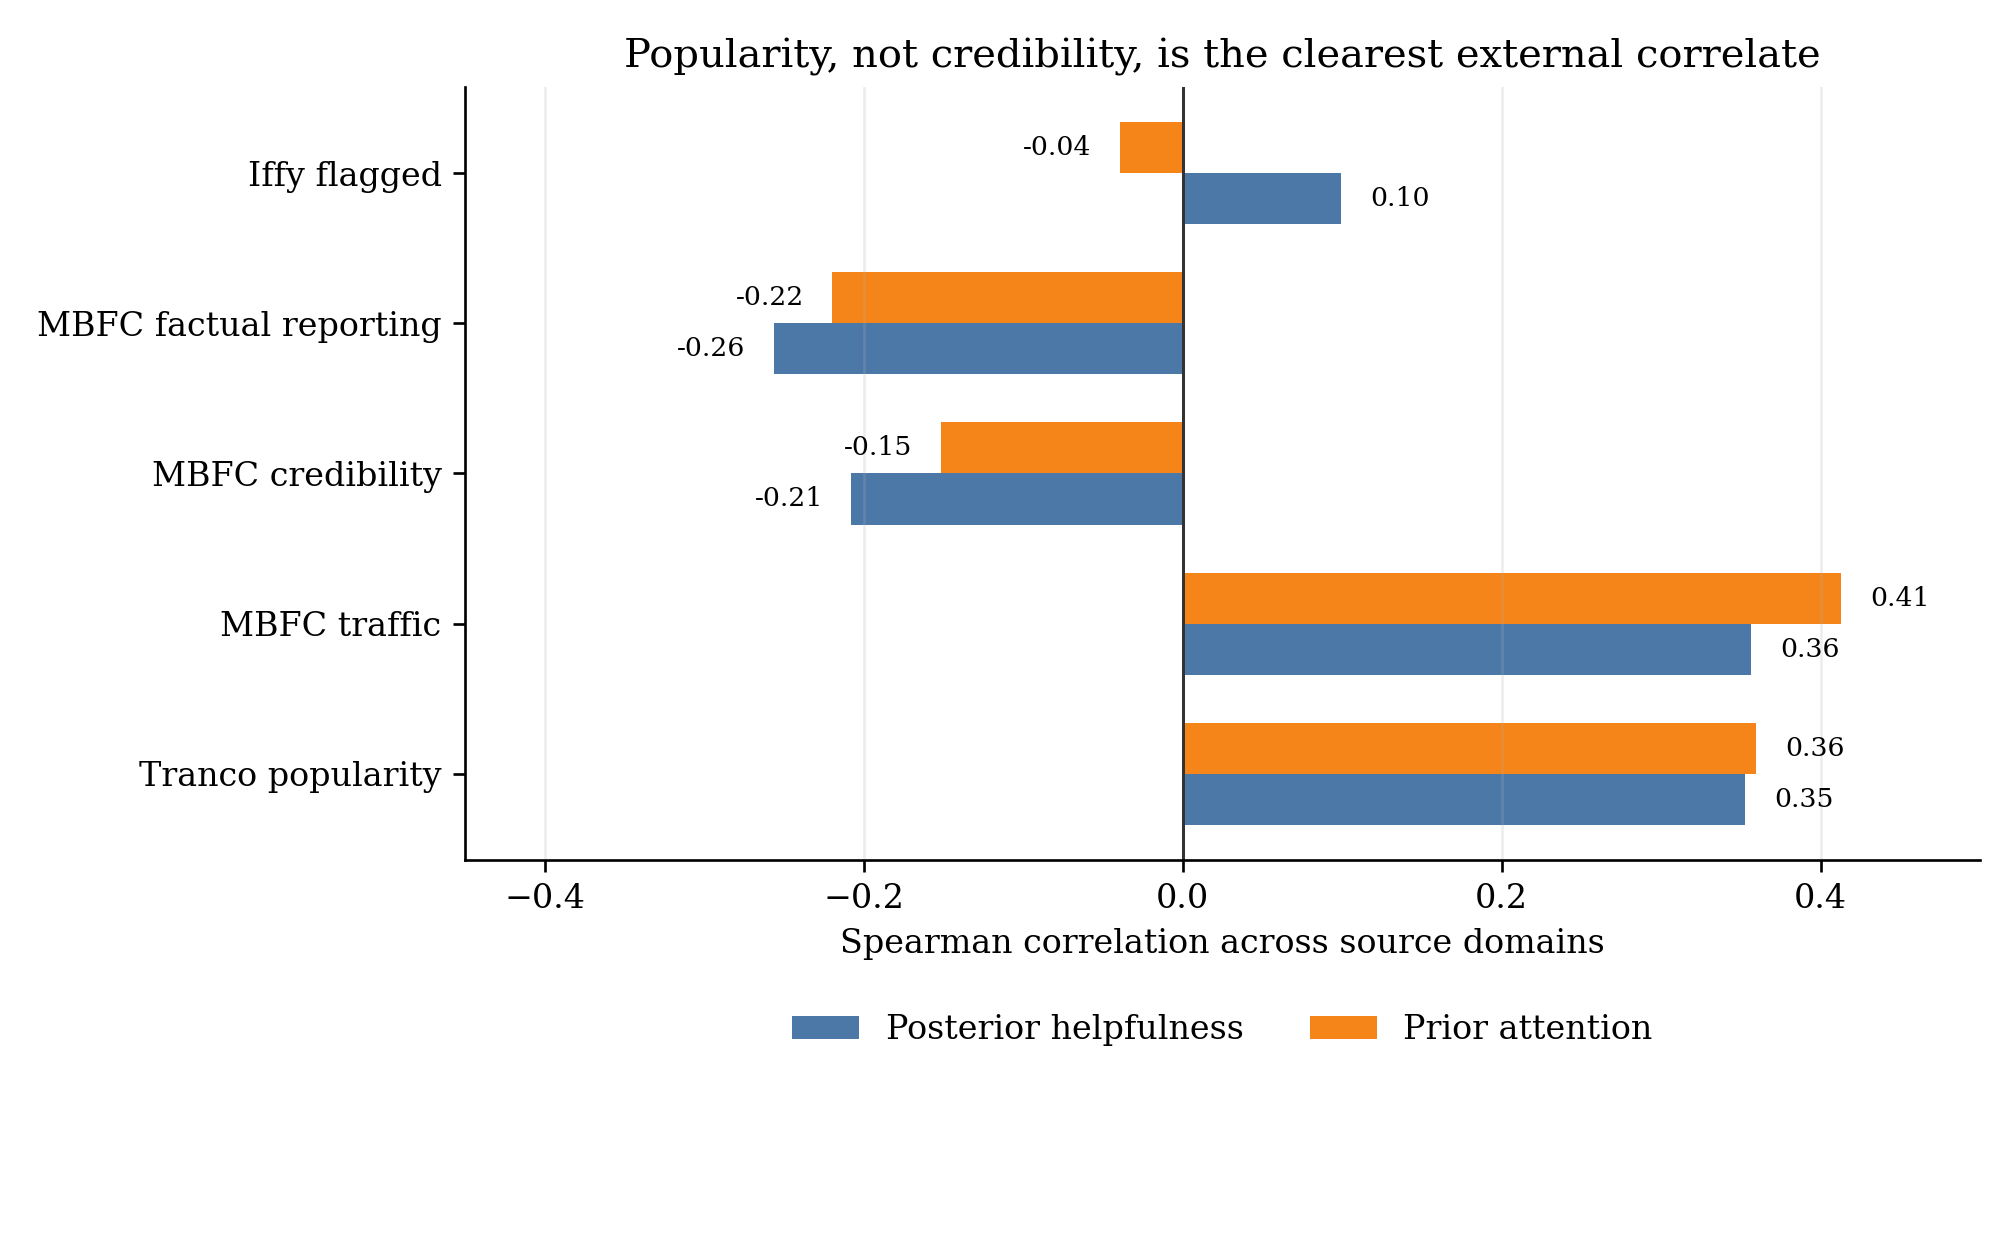
\includegraphics[width=0.92\linewidth]{fig2_source_attribute_correlations.png}
\caption{Bars are unadjusted Spearman correlations across source domains. Positive values mean domains higher on the attribute also have higher average posterior helpfulness or prior attention. Popularity and traffic are positive; MBFC credibility and factual-reporting labels are negative in this raw panel. These are descriptive correlations, not causal estimates.}
\label{fig:source-correlations}
\end{figure}
\begin{table}[H]
\centering
\caption{Unadjusted source-attribute correlations.}
\small
\resizebox{\linewidth}{!}{%
\begin{tabular}{p{0.3\linewidth}p{0.28\linewidth}rr}
\toprule
Predictor & Outcome & Domains & Spearman \\
\midrule
Tranco attention & Posterior helpfulness & 348 & 0.353 \\
Tranco attention & Prior attention & 348 & 0.360 \\
MBFC credibility & Posterior helpfulness & 257 & -0.208 \\
MBFC credibility & Prior attention & 257 & -0.152 \\
MBFC reporting & Posterior helpfulness & 257 & -0.256 \\
MBFC reporting & Prior attention & 257 & -0.220 \\
MBFC traffic & Posterior helpfulness & 257 & 0.356 \\
MBFC traffic & Prior attention & 257 & 0.413 \\
Iffy flag & Posterior helpfulness & 351 & 0.100 \\
Iffy flag & Prior attention & 351 & -0.039 \\
\bottomrule
\end{tabular}
}
\caption*{\footnotesize Spearman correlations are computed across source domains with at least 20 candidate articles. These are descriptive correlations, not causal effects.}
\label{tab:source-correlations}
\end{table}

\section{Finding 2: Source-Level Attention and Helpfulness Move Together}
The external-source result is consistent with the model's own source-level behavior. Among source domains with at least 20 candidate articles, mean prior attention $A_d$ and mean posterior helpfulness $H_d$ have Spearman correlation \DomainPriorPosteriorSpearman\ (Pearson \DomainPriorPosteriorPearson). In other words, domains that receive more learned attention also tend to be domains whose articles receive more hindsight attribution. This is a source-level association, not proof that popularity or credibility caused the market move.
\begin{figure}[H]
\centering
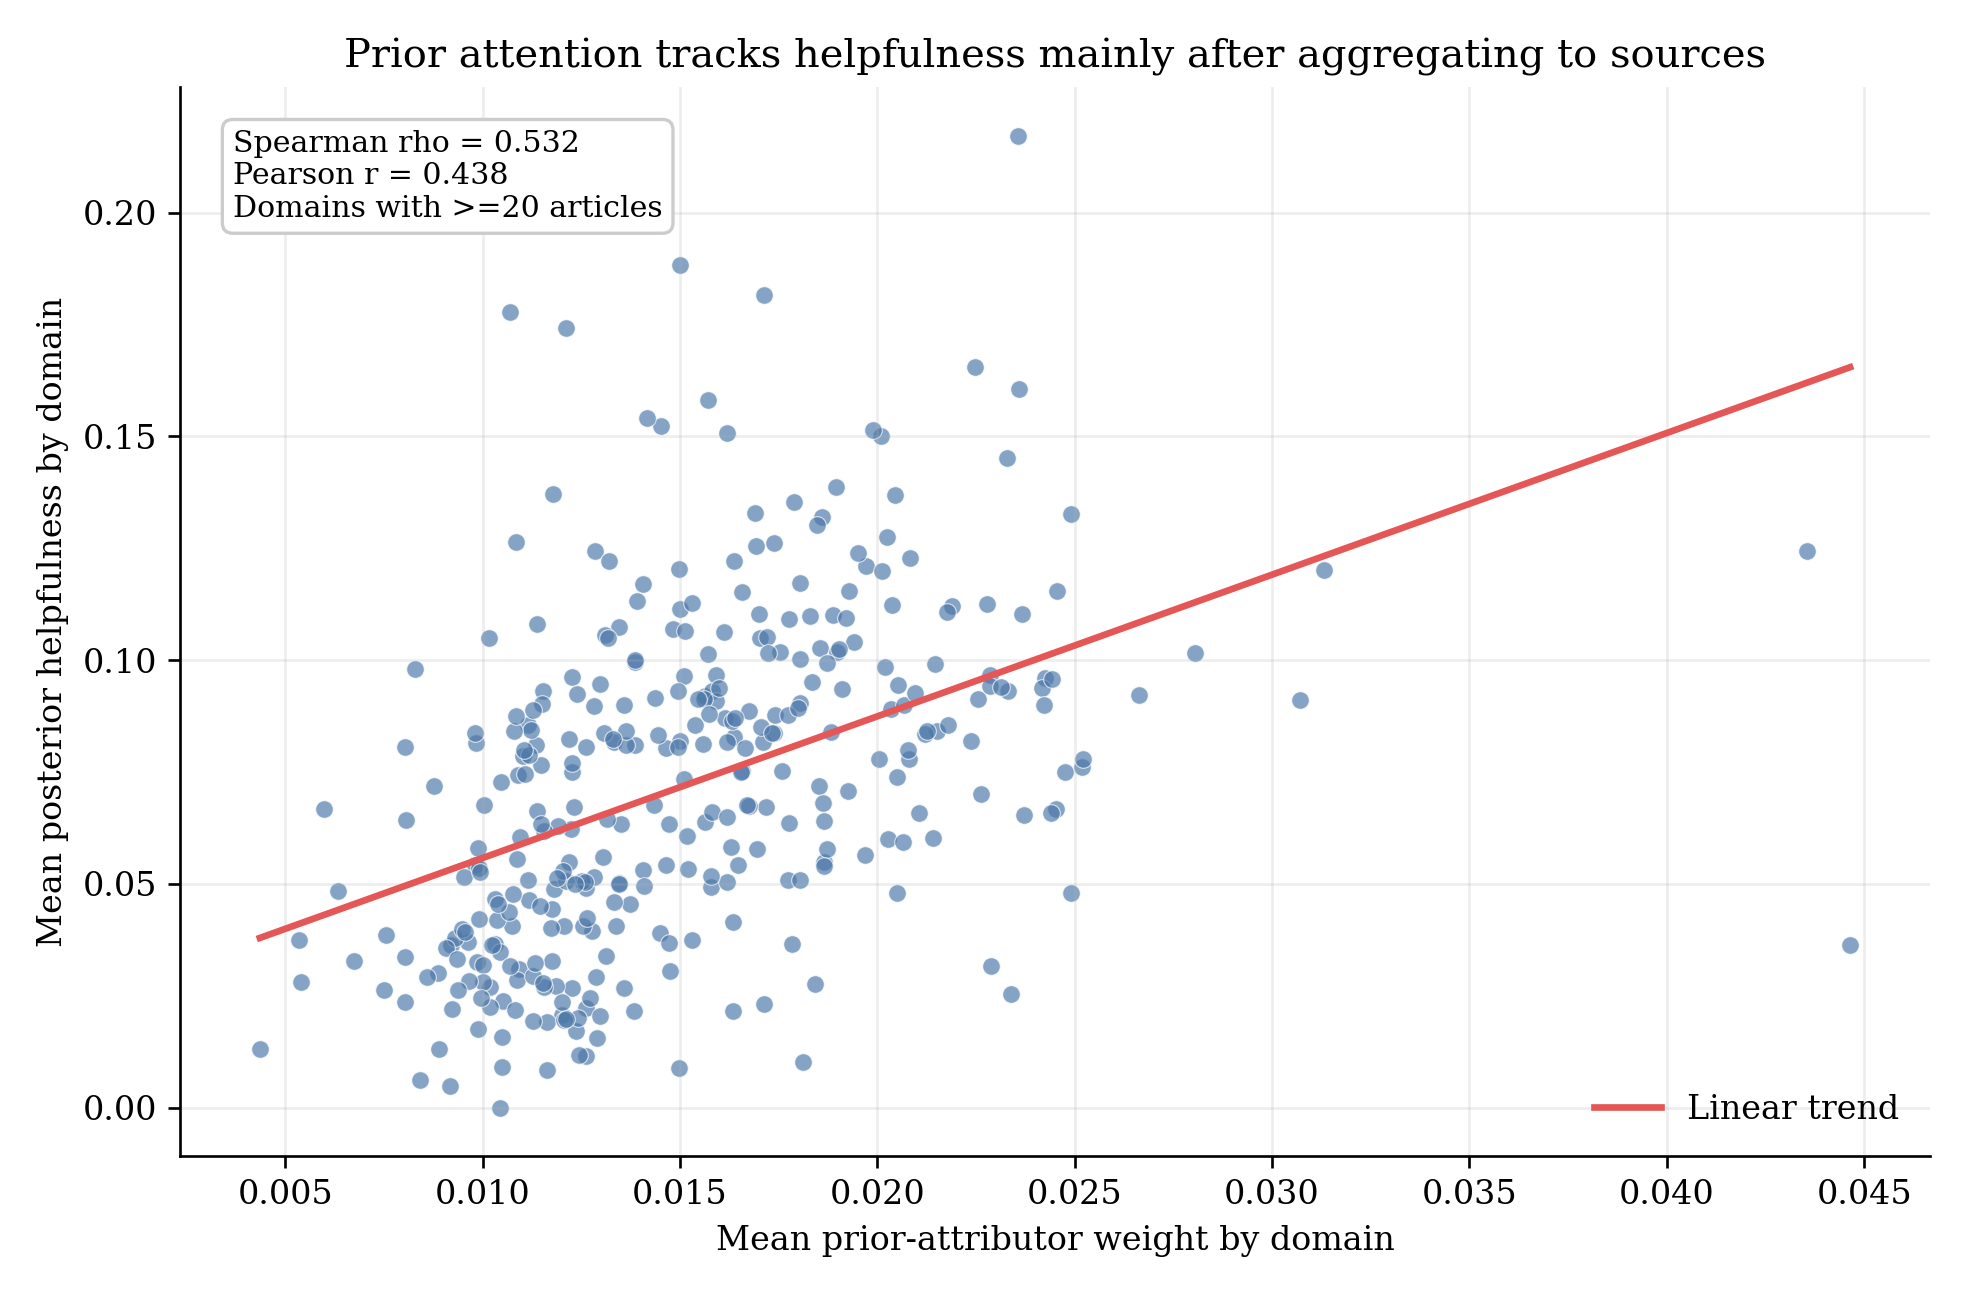
\includegraphics[width=0.92\linewidth]{fig1_domain_prior_vs_posterior.png}
\caption{Each dot is a source domain with at least 20 candidate news articles. The horizontal axis is the domain's mean prior-attributor weight $A_d$; the vertical axis is its mean posterior helpfulness $H_d$. The positive trend shows that source-level averages line up, but it does not show causal influence or faithful item-level explanation.}
\label{fig:domain-prior-posterior}
\end{figure}
\section{Finding 3: Source Patterns Are Not Item-Level Explanations}
The source-level correlations are easier to interpret after checking the item-level attribution behavior. Because $P_\eta$ is trained to approximate posterior attributions, some relationship between $q_{ri}$ and $s_{ri}$ is expected. At the candidate-news level it is weak: among held-out records with any posterior-positive news, the item-level Spearman correlation between $q_{ri}$ and $s_{ri}$ is \TestItemPositiveRecordSpearman. The prior selects useful candidates more often than chance, but exact recovery of the hindsight top item remains low at \TestPriorExactTopRate.
\begin{table}[H]
\centering
\caption{How closely does the learned prior attributor match posterior helpfulness?}
\small
\resizebox{\linewidth}{!}{%
\begin{tabular}{lll}
\toprule
Check & Estimate & Read \\
\midrule
Item ranking & test rho 0.067 & weak item faithfulness \\
Within-record ranking & test mean rho 0.084 & weak but positive \\
Mass on positive news & test mean 0.505 & useful, not oracle \\
Top item nonzero & test 61.9\% & often relevant \\
Exact top match & test 16.2\% & low recovery \\
Domain averages & domain Spearman 0.532 & stronger aggregated \\
\bottomrule
\end{tabular}
}
\caption*{\footnotesize q is the released prior-attributor score; posterior-positive means the hindsight/posterior score s is greater than zero. Test estimates use held-out Kalshi records.}
\label{tab:prior-signal}
\end{table}

\section{Interpretation}
The results support a careful version of the attention-is-not-information claim. Source popularity is a useful predictor of both learned attention and hindsight helpfulness in this release; credibility labels are not. But these are source-level regularities, not causal estimates and not faithful explanations of which exact article mattered. A system can learn where useful information often comes from without reliably explaining which particular item drove a belief update.
\section{What This Does Not Answer}
This report does not establish that a source caused a market move. It also does not test forecast-community rationales, likes, comments, author reputation, or market microstructure. Those require a Manifold- or Metaculus-style dataset with written rationales, engagement metrics, timestamps, price movement around each rationale, and final resolution. The SWM news analysis is best read as a reproducible baseline for that later rationale-level design.
\clearpage
\appendix
\section{Provenance and Reproducibility}
The report was generated without new LLM calls. The two analysis scripts were:
\begin{quote}
\small\texttt{scripts/build\_source\_attribute\_panel.py}\\
\small\texttt{scripts/generate\_no\_training\_report.py}
\end{quote}
The latter compiles this TeX source with the bundled Tectonic engine. The bundle includes this TeX file, a rendered PDF, figures, CSV tables, generated TeX tables, numeric macros, a Markdown report, and provenance JSON.
\section{Known Limits}
No new LLM training or inference was run. The released Kalshi data contain candidate news, not forecast-community rationales. The posterior attribution scores are hindsight labels and should not be interpreted as formal causal proof. Actual random-news forecast harm cannot be scored without unreleased prediction outputs or a rerun of the trained world model; the available no-training proxy found a \RandomTopOneZeroMissRate\ random top-one zero-miss rate among high-attribution records.
\section{References}
\begin{itemize}
\item Yu et al. (2026), \textit{Building Social World Models with Large Language Models}: \url{https://arxiv.org/pdf/2606.11482}
\item SWM-Bench dataset: \url{https://huggingface.co/datasets/ulab-ai/swm-bench}
\item Social World Model code: \url{https://github.com/ulab-uiuc/social-world-model}
\item Tranco: \url{https://tranco-list.eu/}
\item Iffy Index: \url{https://iffy.news/index/}
\item MBFC extension data: \url{https://github.com/drmikecrowe/mbfcext/}
\end{itemize}
\end{document}
